
\chapter{Method}
	
	Points within a 3d point cloud are simply represented by their x, y, z Cartesian coordinates. This means that there is a possibility that there are two points with the same x, y, z coordinates that have been acquired at different times, this is assuming that the origin is the same. Comparing these points is not as easy as one would assume, they may occupy the same point in space, but cannot simply assume that they are the same.
	
	We may get some extra data from a laser scanner, such as intensity and colour. But this doesn't really give us any information about the area surrounding these points and weather anything has changed.
	
	Situations where points need to be compared for any reason require more information than can be provided by a laser scanner. So the idea of looking at each point individually now falls away. We need to start looking at the bigger picture of what the point cloud is telling us.\\
	\\
	Machine learning is a subfield of computer science that evolved from pattern recognition and learning theory in artificial intelligence. it is in the field of machine learning that we start to look at the bigger picture of what our point clouds are telling us. Machine learning is the study of creating algorithms that can learn from and make predictions about data.\\
	\\
	The aim of this Thesis is, given an uncleaned, noisy point cloud of a room to create an .obj file with lines representing all the edges of that room.
	
	
\section{Segmentation}

	\subsection{Principal Components Analysis}
		A Principal Components Analysis (PCA) is the default method for estimating normals in Point Cloud Library. it is the fastest method because of PCL's multi-threading option for the function.
		
		A principal components analysis can be thought of as fitting an \textit{n}-dimensional ellipse to a set of data. Each axis of the ellipse represents a principal component. If an axis is large then the variance along that axis is large, and vice versa. When calculating the normal of a point set, the smallest axis is the axis with with the least variance and therefore represents the normal. This is easy to think of with a 2D disk of points, like in figure \ref{fig:PCA2D Example}. Its easy to see how the 3rd axis for these set of point will be coming out of the page, as it has to be orthogonal to the other two.
		
		\begin{figure}[H]
			\centering
			\begin{subfigure}{.5\textwidth}
				\centering
				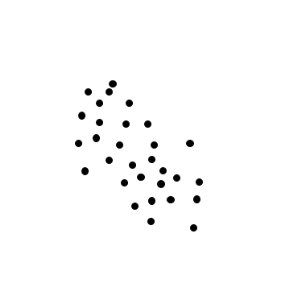
\includegraphics[width=1\linewidth]{Includes/images/pca1}

				\label{fig:sub1}
			\end{subfigure}%
			\begin{subfigure}{.5\textwidth}
				\centering
				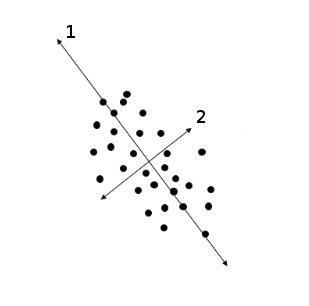
\includegraphics[width=1\linewidth]{Includes/images/pca2-ver2}

				\label{fig:sub2}
			\end{subfigure}
			\caption{A 2D representation of a Principal Components Analysis }
		\end{figure} 
		
		To fit this \textit{n}-dimensional ellipse we compute the covariance matrix of the data set and calculate the eigenvalues and corresponding eigenvectors of this covariance matrix.
		
		\subsubsection{Calculating the Covariance Matrix of a given set of 3D points}
			The covariance matrix, $C$, is calculated for each point $p_i$ as follows:
			
			\begin{equation}
			C = \frac{1}{k} \sum_{i=1}^{k}.(p_i - \bar{p}).(p_i - \bar{p})^T
			\end{equation}
			
			Where $k$ is the number of points in the neighborhood of point $p_i$, and $\bar{p}$ is the 3D centroid of the nearest neighbors.
				
		\subsubsection{Calculating Eigenvalues and Eigenvectors}
			Eigenvalues, $\lambda_j$, and eigenvectors, $\vec{v_j}$, are calculated on the covariance matrix, $C$, for a given point:
			
			\begin{equation}
			C \vec{v_j} = \lambda_j \vec{v_j}
			\end{equation}
			After solving the system and getting results for $\lambda_j$ and $\vec{v_j}$, the smallest eigenvalue and its corresponding eigenvector is are as the normal $\vec{n_i}$ for that point.\\
			\\
			\\
			There is no mathematical method for determining the sign of the normal, its orientation as computed in the PCA is ambiguous, and not consistent over the whole point cloud. 
			
			The solution to this issue is simple. If the viewpoint is known, in the case of laser scans the scan center, then orientate all normals $\vec{n_i}$ towards the viewpoint. This whole process results in what is seen in figure \ref{fig:Normals}.
			
			\begin{figure}[H]
			\centering
			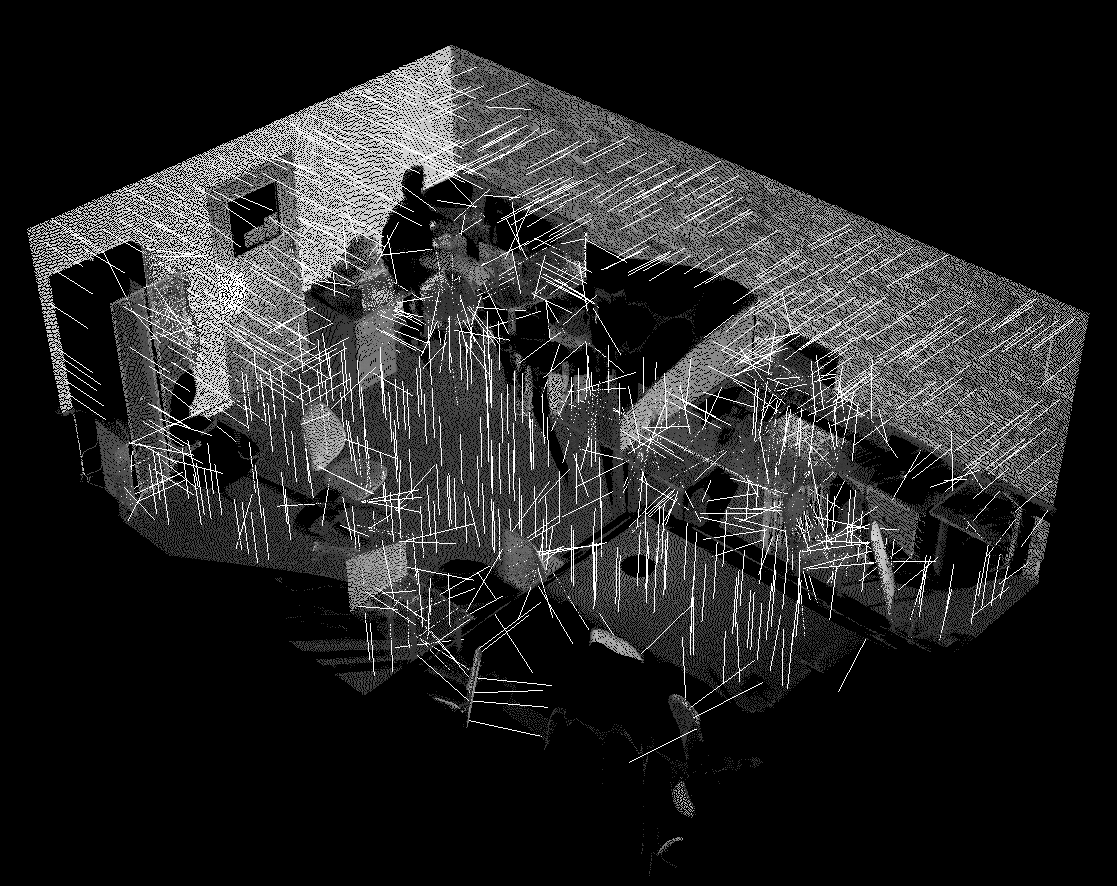
\includegraphics[width=0.7\linewidth]{Includes/images/Normals}
			\caption{Normals calculated over a cut down section of a point cloud (the roof has been removed for ease of viewing)}
			\label{fig:Normals}
			\end{figure}
		

				
	\subsection{Region Growing}
	
		Once the normals have been calculated a region growing algorithm is executed.
		
		The Region growing algorithm starts off by selecting seed points. This is done by calculating the curvature of each point then storing all the points in an array, sorted by their curvature value. The reason for this is because the point with the least curvature associated with it is located in the flattest section of the point cloud. Now regions can begin to be grown using the flattest points in the cloud as seed points. 
		
		The first point in the sorted array is chosen as the first seed point:
		
		\begin{itemize}
			
			\item The nearest neighbors to this point are looked at and are either rejected or accepted into the region based on user defined criteria such as normal deviation and smoothness and curvature constraints.
			
			\item Once a point is accepted into the region, the process starts again based on that point.
			
			\item Once no more points are found for that particular seed, or the region reached a specified maximum, the seed is removed from the set of seeds and the region is added to the global segment list. 
			
		\end{itemize}
		
		This is repeated while the list of available points is not empty.
		
		If after a seed point has been through the process and the number of points does not reach the user defined minimum size, the region removed from the cloud as unclassified. Unclassified points are removed from the cloud completely after the process is terminated.
		
		\begin{figure}[H]
			\centering
			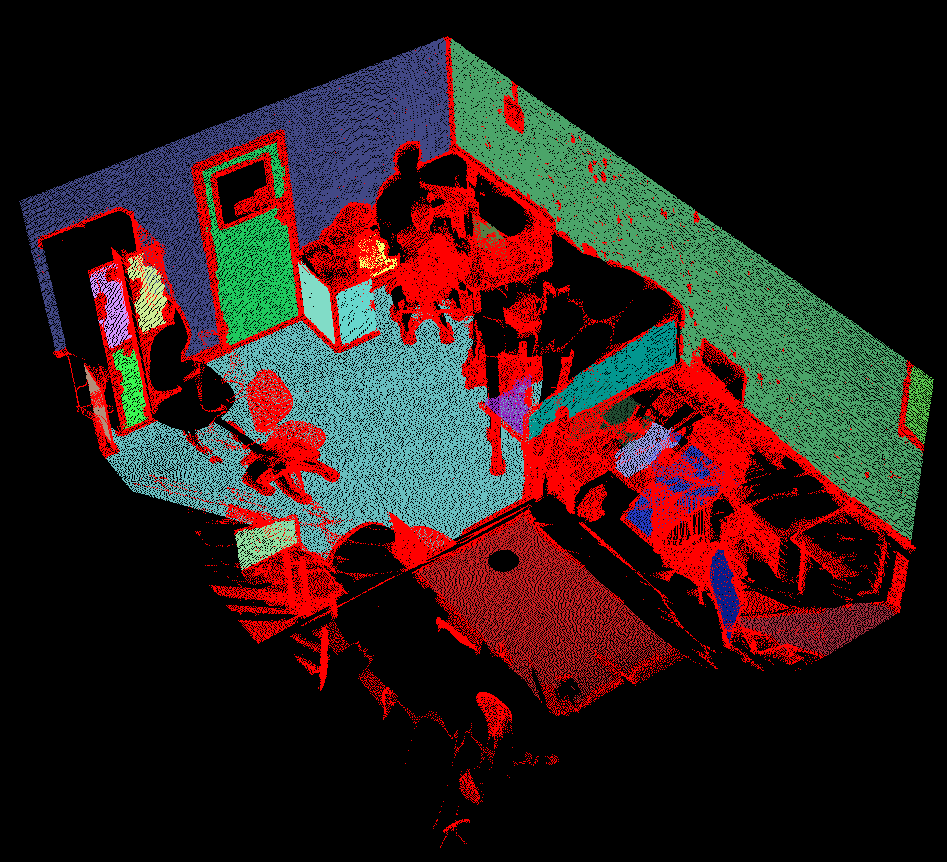
\includegraphics[width=0.6\linewidth]{Includes/images/GrownRegions}
			\caption{Red Points represent unclassified points}
			\label{fig:GrownRegions}
		\end{figure}
		
		The unclassified points are of no use, and are therefore removed.
		
		
		\begin{figure}[H]
			\centering
			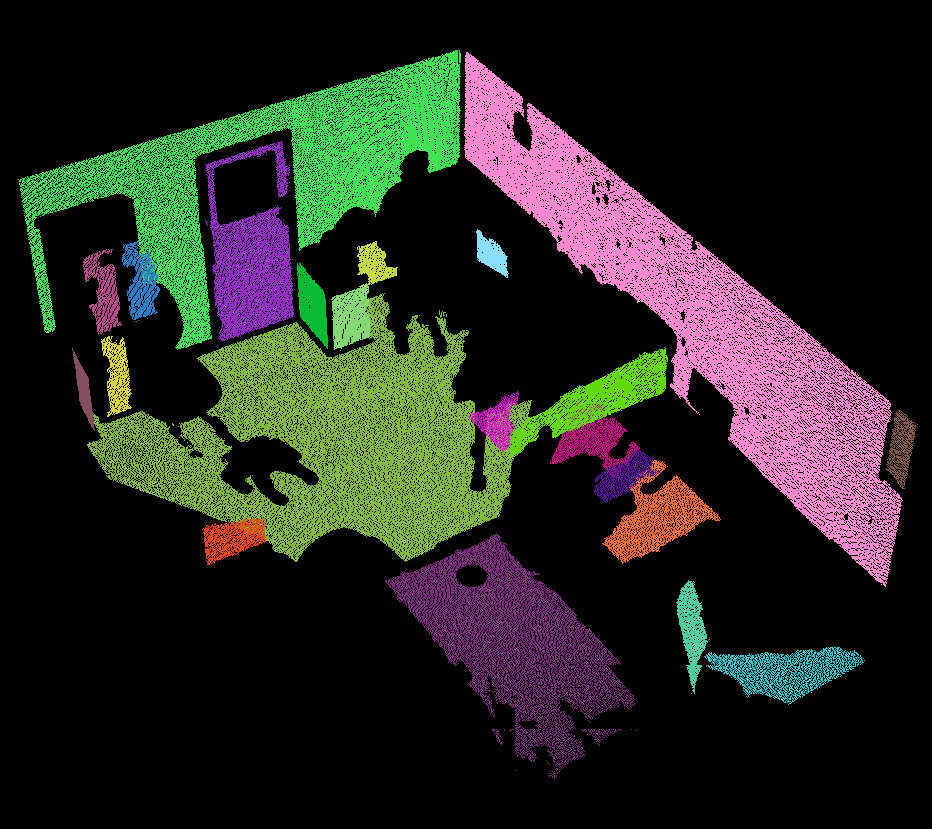
\includegraphics[width=0.6\linewidth]{Includes/images/RG-noUnclass}
			\caption{Segmented room with unclassified points removed}
			\label{fig:RG-noUnclass}
		\end{figure}
		
		
		It is important to note that for the application of this paper the segments have to be planar, therefore very strict parameters were used to make sure that the segments did not have curvature in them.\\
		\\
		A pseudo-code algorithm for region growing can be found in appendix A.
		
	
\section{Surface Extraction}
	It is immediately evident in Figure \ref{fig:RG-noUnclass} that there are too many small segments that are not necessary and irreverent to the final output. So it becomes necessary to filter these segments out.
	
	To begin this, a vector of the segments is created after the region growing has taken place.
	
		\subsection{Random Sample Consensus}
			When looking at an individual segment the calculated normals no longer have any relevance, it becomes necessary to stop looking at the points that make up a segment and rather look at the segment as a whole. 
			
			For this Random Sample consensus (RANSAC) is used to estimate a normal to the segment by fitting a plane to it.
			
			RANSAC achieves this goal by iteratively selecting a random subset of the original data, this subset of the original data is considered inliers. A model is fitted and the hypothesis that this is the correct model is then tested as follows:
			
			\begin{enumerate}
				\item All other data is then tested against this model, if a point fits well it is considered a hypothetical inlier.
				
				\item The model is considered a reasonably good fit if enough points are considered inliers.
				
				\item The model is then re-estimated from all hypothetical inliers, as opposed to only the initial set.
				
				\item Then finally the model is evaluated by calculating the error of all the points relative to the model.
			\end{enumerate}
			
			This process is repeated a fixed number of times, each time either rejecting the model if there are too few inliers, or replacing the last saved model if the error is lower.
			\subsubsection{Choosing number of iterations in RANSAC method}
			$k$ (the number of iterations) required for a successful estimation within a certain probability can be calculated:
			
			\begin{equation}
				k = \frac{\log(1-p)}{\log(1- w^n)}
			\end{equation}
			
			where P(success) = $p$ and P(Selecting an inlier) = $w$ and $n$ = the points that are needed to create the initially estimated model(in 3D case of plane fitting $n = 3$)\\
			\\
			$w$ is usually not known but a rough estimate can be found.\\
			\\
			
			Below is a 
		
			\begin{figure}[H]
				\centering
				\begin{subfigure}{.5\textwidth}
					\centering
					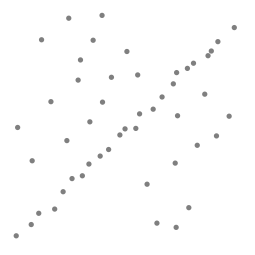
\includegraphics[width=1\linewidth]{Includes/images/random_sample_example1}
					\label{fig:RANSAC1}
				\end{subfigure}%
				\begin{subfigure}{.5\textwidth}
					\centering
					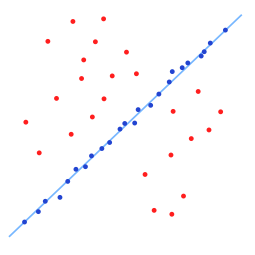
\includegraphics[width=1\linewidth]{Includes/images/random_sample_example2}
					\label{fig:RANSAC2}
				\end{subfigure}
				\caption{A 2D representation of RANSAC showing inliers in blue and outliers in red}
			\end{figure} 
		 
			
			A pseudo-code algorithm for RANSAC can be found in appendix A.
		\subsection{Segment selection}

			
			\subsubsection{filtering out Horizontal and Vertical surfaces}
				The vector of segments created in the segmentation section of the program is not entirely useful because \\
				\\
				fit plane\\
			\\
				Once a plane has been fitted to the segment the normal to that segment is said to be the coefficients $a$, $b$, and $c$ of the plane equation.\\
				\\
				split based on orientation
			



\section{Model Generation}
		\subsection{Bounding Box Generation}
		OBB
		Moment of inertia
		
		\subsection{Angle between Planes}
		
		\subsection{Plane with Plane Intersection}
		
		\subsection{Orthogonal Distance of point to line}
		
		\subsection{Project points onto line}
		
		\subsection{Create OBJ file}

	


